\begin{enumerate}[label=\thesection.\arabic*.,ref=\thesection.\theenumi]
\numberwithin{equation}{enumi}
\renewcommand{\thefigure}{\theenumi.\arabic{figure}}

\item For the circuit in Fig. \ref{fig:ee18btech11050_f1} (ignore the amplitude stabilization circuitry), find the loop gain GH by breaking the circuit at node X. 

\begin{figure}[!ht]
	\begin{center}
		\resizebox{\columnwidth}{!}{\begin{circuitikz}
\ctikzset{bipoles/length=1cm}

\draw 
(0, 0) node[op amp] (opamp) {}
(opamp.-) -- (-2.5,0.35) to[R,l_=$10k\ohm$,*-*] (-3.5, 0.35) to [C,l_=$16nF$,*-*] (-5,0.35) to [C,l_=$16nF$,*-*] (-6, 0.35) to [C,l_=$16nF$,*-*] (-7, 0.35) {}
(opamp.+) -- (-1.0,-0.35) node[ground]{}
(-4.8,0.35) -- (-4.8,-0.8) to [R,l_=$R$,*-*](-4.8,-1.8) --(-4.8,-2.3)node[ground] {}
(-6,0.35) -- (-6,-0.8) to [R,l_=$R$ ,*-*](-6,-1.8) --(-6,-2.3) node[ground] {}
(opamp.-) -- (-0.9,1.5) to [D, l_=$D_1$, *-*](1,1.5)to [R,l_=$R_2$, *-*](1,0.25)--(1,0){}
(1,0) to[R,l_=$R_3$, *-*](1,-2)to[D,l_=$D_2$,*-*](-1,-2)--(-2,-2) --(-2,0.35){}
(1,-2) to[R,l_=$R_4$, *-*](1,-4) node[vee]{$V^-$}
(1,1.5) to[R,l_=$R_1$, *-*](1,3) node[vcc]{$V^+$}
(opamp.out) to (2.5,0)--(2.5,7) -- (-7,7) -- (-7,0.35){}
(2.5,0)--(3,0){}
(2.5,0)--(2.5,5) to [potentiometer,n=mypot,l_=$P_1$](0.5,5) to  [R,l=$100k\ohm$](-0.6,5) --(-0.9,5)--(-0.9,1.5){}
(mypot.wiper) --(2,4.6)  --(2,5){}

(-0.3,5.5)coordinate(left)
(2,5.5)coordinate(right)
(-0.3,4.8)coordinate(bottoml)
(2,4.3)coordinate(bottomr)

node[fit=(left)(right)(bottoml)(bottomr),draw, dashed, label={$R_f$},inner sep=10pt] {}
node at(3.3,0){$V_0$}
node at(-7.5,0.1){$X$}
node at(-4.1,-1.5){$10k\ohm$}
node at(-6.6,-1.8){$10k\ohm$}
node at(-3,-0.1){$R$}
node at(-4.2,-0.2){$C$}
node at(-5.5,-0.2){$C$}
node at(-6.5,-0.2){$C$}
;\end{circuitikz}
}
	\end{center}
\caption{}
\label{fig:ee18btech11050_f1}
\end{figure}

\item \solution
The equivalent control system representation of Oscillator circuit is shown in Fig. \ref{fig:ee18btech11050_f4}. Oscillator circuits do not have input.
\begin{figure}[!ht]
	\begin{center}
		\resizebox{\columnwidth}{!}{\input{./figs/ee18btech11050/blockdiagram.tex}}
	\end{center}
\caption{}
\label{fig:ee18btech11050_f4}
\end{figure}
After removing the amplitude stabilization circuitry, when we break the loop at X, from Fig. \ref{fig:ee18btech11050_f2} the value of gain
\begin{align}
    GH = \frac{v_o(j\omega)}{v_x(j\omega)}
\end{align}

\begin{figure}[!ht]
	\begin{center}
		\resizebox{\columnwidth}{!}{\begin{circuitikz}
\ctikzset{bipoles/length=1cm}

\draw 
(0, 0) node[op amp] (opamp) {}
(opamp.-) -- (-1.5,0.35) to[R,l_=$R$,*-*] (-2.5, 0.35) to [C,l_=$C$,*-*, i<=$i_x$] (-4,0.35) to [C,l_=$C$,*-*] (-5.5, 0.35) to [C,l_=$C$,*-*] (-7, 0.35) {}
(opamp.+) -- (-1.0,-0.35) node[ground]{}
(-5.5,0.35) -- (-5.5,-0.8) to [R,l_=$R$,*-*](-5.5,-1.8) --(-5.5,-2.3)node[ground] {}
(-4,0.35) -- (-4,-0.8) to [R,l_=$R$ ,*-*](-4,-1.8) --(-4,-2.3) node[ground] {}
(opamp.out) -- (2,0){}
(2,0)--(3,0){}
(2.5,0)--(2.5,2) to[R, l_=$R_f$, i<=$i_x$](-1,2) --(-1,2)--(-1,0.35){}

node at(3.3,0){$v_o$}
node at(-7,0.1){$v_x$}
node at(0.1,1.5){$+$}
node at(1.2,1.5){$-$}
node at(-1,0.1){$v_1$}
node at(-4, 0.6){$v_a$}
node at(-5.5, 0.6){$v_b$}

;\end{circuitikz}
}
	\end{center}
\caption{}
\label{fig:ee18btech11050_f2}
\end{figure}
\begin{align}
    v_1 = 0
\end{align}
\begin{align}
    \implies v_o = -i_xR_f
    \label{ee18btech11050_eq1}
\end{align}
\begin{align}
    v_a = (\frac{1+sRC}{sC})i_x
\end{align}
\begin{align}
    \implies v_b = (R + \frac{3}{sC} + \frac{1}{s^2C^2R})i_x
\end{align}
\begin{align}
    \implies v_x = (R + \frac{6}{sC} + \frac{5}{s^2C^2R} + \frac{1}{s^3C^3R^2})i_x
\end{align}

\begin{align}
    \implies\frac{v_x}{i_x} = (R+\frac{6}{sC}+\frac{5}{s^2C^2R}+\frac{1}{s^3C^3R^2})
\end{align}
From \eqref{ee18btech11050_eq1}
\begin{align}
    \frac{v_x}{v_o} = -\frac{R}{R_f}(1+\frac{6}{sCR}+\frac{5}{s^2C^2R^2}+\frac{1}{s^3C^3R^3})
\end{align}

\begin{align}
    \implies \frac{v_o}{v_x} = -\frac{R_fs^3C^3R^3}{R(s^3C^3R^3+6s^2C^2R^2+5sCR+1)}
\end{align}
Substituting $s=j\omega$ gives us the transfer function
\begin{align}
    \frac{v_o}{v_x} = GH = \frac{\omega^2C^2R_fR}{(5-\omega^2C^2R^2)+j(6\omega CR-\frac{1}{\omega CR})}
    \label{ee18btech11050_eq2}
\end{align}

\item Find frequency of oscillation $f_0$.
\item \solution 
For system to oscillate at a frequency $\omega_0$, 
\begin{align}
    L(j\omega_0) = G(j\omega_0)H(j\omega_0) = 1
    \label{ee18btech11050_eq4}
\end{align}
\begin{align}
    \implies \angle(G(j\omega_0)H(j\omega_0)) = 0
\end{align}
\begin{align}
    \implies 6\omega_0 CR = \frac{1}{\omega_0 CR}
\end{align}
\begin{align}
    \implies \omega_0 = \frac{1}{\sqrt{6}CR}
\end{align}
\begin{align}
    \implies \omega_0 = 2551.55 rad/sec
\end{align}
\begin{align}
    \implies f_0 = 406.1 Hz
\end{align}
\item Find $R_f$ for oscillation to begin.
\item \solution From \eqref{ee18btech11050_eq4}
\begin{align}
    Re(G(j\omega_0)H(j\omega_0)) = 1
\end{align}
\begin{align}
    \implies \frac{R_f\omega_0^2C^2R}{5-\omega_0^2C^2R^2} = 1
\end{align}
\begin{align}
    \implies R_f = 29R
\end{align}
\begin{align}
    \implies R_f = 290 k\ohm
\end{align}
Thus, for the oscillations to begin,
\begin{align}
    R_f \geq 290 k\ohm
\end{align}
\item Tabulate your results.
\item \solution See table \ref{parameters}
\begin{table}[!ht]
\centering
\input{./tables/ee18btech11050/table1.tex}
\caption{calculated parameters}
\label{parameters}
\end{table}

\item Verify results using Spice Simulation.

\item \solution Following readme provides instructions for simulation in spice

\begin{lstlisting}
codes/ee18btech11050/spice/README.md
\end{lstlisting}

The following netlist simulates the given circuit in \ref{fig:ee18btech11050_f1}

\begin{lstlisting}
codes/ee18btech11050/spice/ee18btech11050_sim.net
\end{lstlisting}

The following code plots the oscillator output from spice simulation, which is shown in fig \ref{fig:ee18btech11050_f6}

\begin{lstlisting}
codes/ee18btech11050/spice/ee18btech11050_sim.py
\end{lstlisting}

\begin{figure}[!ht]
\centering
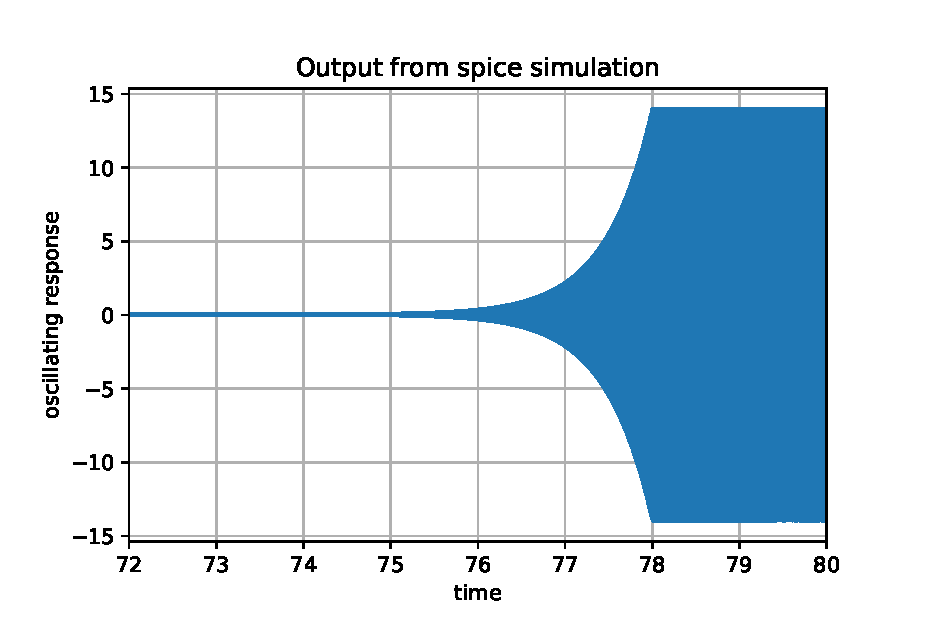
\includegraphics[width=\columnwidth]{./figs/ee18btech11050/ee18btech11050_sim.eps}
\caption{}
\label{fig:ee18btech11050_f6}
\end{figure}

The following code plots a part of spice output generated above, where a sinusoidal output can be clearly observed shown in fig \ref{fig:ee18btech11050_f7}

\begin{lstlisting}
codes/ee18btech11050/spice/ee18btech11050_sim2.py
\end{lstlisting}

\begin{figure}[!ht]
\centering
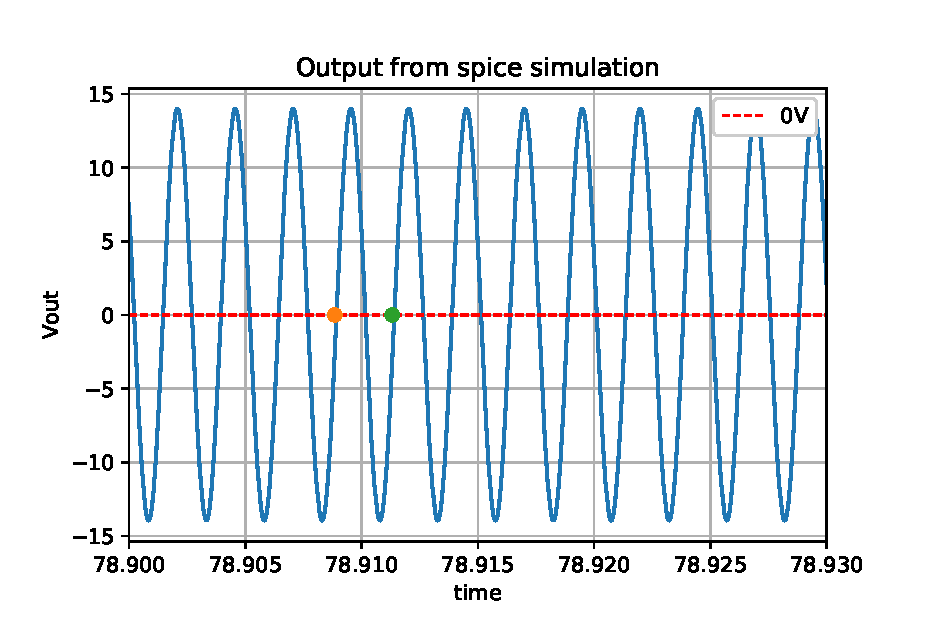
\includegraphics[width=\columnwidth]{./figs/ee18btech11050/ee18btech11050_sim2.eps}
\caption{}
\label{fig:ee18btech11050_f7}
\end{figure}

From fig \ref{fig:ee18btech11050_f7}, time period is calculated from one cycle:
\begin{align}
    T = 78.91131 - 78.908846 = 0.002464 sec
\end{align}
\begin{align}
    \implies f = 405.844 Hz
\end{align}

Hence frequency is verified through spice simulation.

\end{enumerate}
